\documentclass[openany]{book} % oppure \openany in mezzo al libro
\usepackage[utf8]{inputenc}
\usepackage[italian]{babel}
\usepackage[T1]{fontenc}
\usepackage{natbib}
\usepackage{amsmath}
\usepackage{latexsym}
\usepackage{geometry}
\usepackage{amsfonts}
\usepackage{multicol}
\usepackage[none]{hyphenat}
\usepackage{blindtext}
\usepackage{graphicx}
\usepackage{enumitem}
\usepackage{old-arrows}
\usepackage{wrapfig}
\usepackage{pdfpages}

\DeclareMathSymbol{\nrightarrow} {\mathrel}{AMSb}{"39}


\sloppy
%\raggedright 
 \geometry{
 a4paper,
 left=20mm,
 right=20mm,
 top=20mm,
 bottom=20mm,
}

\newcommand{\ind}{\mathrel{\text{\scalebox{1.07}{$\perp\mkern-10mu\perp$}}}}

\pagestyle{empty}

\title{Titolo}
\date{}
\author{MT}
\renewcommand{\baselinestretch}{1.2}

\setlength{\parindent}{0em}
%\setlength{\parskip}{0.2em}

\setlist{nosep}

\begin{document}

\begin{center}
	\Large Probabilità e Statistica

	\large Formulario
\end{center}

$e^{ix} = \cos(x)+i\sin(x) \quad e^x = \underset{n \rightarrow\infty}{\text{lim}}\left(1+\frac{x}{n}\right)^n \quad e^x=\sum_{n=0}^\infty \frac{x^n}{n!}$

\textbf{Disposizioni con ripetizione} $D^R_{n.k}=n^k$

\textbf{Disposizioni semplici} $D_{n,k}=\frac{n!}{(n-k)!}$

\textbf{Permutazioni di n elementi} \quad $P_n = D_{n,n}=n!$

\textbf{Combinazioni semplici} (numero di sottoinsiemi di cardinalità $k$) \quad $C_{n,k}=\binom {n}{k} = \frac{n!}{k!(n-k)!}$

\textbf{Coefficiente multinomiale} (numero di modi in cui si può partizionare un insieme in $r$ sottoinsiemi di cardinalità $k_1,\dots,k_n$) \quad $\binom {n}{k_1,\dots,k_n}=\frac{n!}{k_1 ! \dots k_n !}$

\textbf{Formula di Poincaré} (principio di inclusione - esclusione) \quad $\mu(A_1 \cup \dots \cup A_n) =$

$= \sum_{k=1}^n (-1)^{k+1}\sum_{1\leq i_1 < \dots <i_k \leq n}\mu(A_{i_1}\cap \dots \cap A_{i_k})$, $\quad \mu$ misura finita

\textbf{Valore atteso} $\mathbb{E}(X) = \int_{-\infty}^{+\infty}xf(x)\,dx$

\textbf{Varianza} $\text{Var}(X)=\mathbb{E}(X^2)-\mathbb{E}(X)^2$

\textbf{Covarianza} $\text{Cov}(X,Y)=\mathbb{E}(XY)-\mathbb{E}(X)\mathbb{E}(Y)$

\textbf{Coefficiente di correlazione} $\rho_{XY} = \frac{\text{Cov}(X,Y)}{\sqrt {\text{Var}(X)\text{Var}(X)}}$

\textbf{Algebra dei valori attesi}

$\mathbb {E}(aX+bY+c)= a\mathbb{E}(X)+b \mathbb{E}(Y)+c$

$\text {Var}(aX+bY+c)= a^2 \text{Var}(X)+b^2 \text{Var}(Y)+2ab\text{Cov}(X,Y)$

$\text{Cov}(aX+bY+c,Z) = a \text{Cov}(X,Z)+b \text{Cov(Y,Z)}$

\textbf{Convoluzione} $X,\,Y$ variabili aleatorie indipendenti, $Z=X+Y$

$f_Z(z) = \int_{-\infty}^{+\infty}f_X(z-y)f_Y(y)\,dy = \int_{-\infty}^{+\infty}f_Y(z-x)f_X(x)\,dx$

\underline{Casi particolari}

\begin{itemize}

	\item $X\sim P(\lambda)\,,\quad Y\sim P(\mu)\Rightarrow Z\sim P(\lambda + \mu)$

	\item $X\sim B(n,p)\,,\quad Y\sim B(m,p)\Rightarrow Z\sim B(n+m,p)$

	\item $X\sim \text{Geo}(p)\,,\quad Y\sim \text{Geo}(p)\Rightarrow Z\sim \text{Pascal}(2,p)$

	\item $X\sim \text{Pascal}(r,p)\,,\quad Y\sim \text{Pascal}(s,p)\Rightarrow Z\sim \text{Pascal}(r+s,p)$

	\item $X\sim \mathcal{N}(\mu_X,\sigma_X^2)\,,\quad Y\sim \mathcal{N}(\mu_Y,\sigma_Y^2)\Rightarrow Z\sim \mathcal{N}(\mu,\sigma^2)$ con $\mu=\mu_X+\mu_Y$ e $\sigma^2=\sigma_X^2+\sigma_Y^2$

	\item $X\sim \Gamma(\alpha,\lambda)\,,\quad Y\sim \Gamma(\beta,\lambda)\Rightarrow Z\sim \Gamma(\alpha+\beta,\lambda)$

	\item $X\sim \text{Exp}(\lambda)\,,\quad Y\sim \text{Exp}(\lambda)\Rightarrow Z\sim \Gamma(2,\lambda)$

	\item $X\sim\chi^2(m)\,,\quad Y\sim\chi^2(n)\Rightarrow Z\sim\chi^2(m+n)$

	\item $X_1,\dots, X_n \sim_{iid} \mathcal{N}(0,1)\Rightarrow X_1^2,\dots, X_n^2 \sim_{iid}\Gamma(\frac{1}{2},\frac{1}{2})\,(\chi^2(1))\Rightarrow Y=X_1^2+\dots+X_n^2\sim\Gamma(\frac{n}{2},\frac{1}{2})$

	      $Y\sim\chi^2(n)$ Chi quadro con $n$ gradi di libertà

\end{itemize}

\begin{multicols}{2}

	\textbf{Bernoulli} $(p)$

	\underline{Densità} $p_X(k) = \begin {cases}1-p & k =0\\ p & k=1\end {cases}$

	\underline{Media} $p$

	\underline{Varianza} $p(1-p)$

	\underline{Funzione di ripartizione} $F_X(k)=(1-p)\, 0\leq k <1 $

	\underline{Funzione caratteristica} $\Phi_X(t)= 1-p+pe^{it}$

	\underline{Commenti} Fallimento e successo
	\\

	\textbf{Binomiale} $(n,p)$

	\underline{Densità} $p_X(k) = \binom {n}{k}p^k(1-p)^{n-k},\,k \in \{0,\dots,n\}$

	\underline{Media} $np$

	\underline{Varianza} $np(1-p)$

	\underline{Funzione caratteristica} $\Phi_X(t)=((1-p)+pe^{it})^n$

	\underline{Commenti} Numero di successi in $n$ lanci con probabilità $p$ di successo
	\\

	\textbf{Multinomiale} $(n,p_1,\dots,p_N)$

	\underline{Densità} $f_{\underline {X}}(n_1,\dots,n_N)=$

	$=\binom {n}{n_1 \dots n_{N+1}}\left(p_1^{n_1}\dots p_N^{n_N}\right)\left(1-\sum_{i=1}^N p_i\right)^{\left(n-\sum_{i=1}^N n_i\right)}=$

	$=\binom {n}{n_1 \dots n_{N+1}}\left(p_1^{n_1}\dots p_N^{n_N}\right)p_{N+1}^{n_{N+1}}$

	\underline{Commenti} $n$ prove ripetute e indipendenti con $N+1$ possibili risultati di probabilità, \quad $p_1,\dots,p_N \Rightarrow$

	$p_{N+1}=1-\sum_{i=1}^Np_i$ ; la marginale della multinomiale è una binomiale
	\\

	\textbf{Pascal} $(p,n)$

	\underline{Densità} $p_X(k) = \binom {n-1}{k-1}p^k(1-p)^{n-k}$

	\underline{Media} $k\frac{1-p}{p^2}$

	\underline{Varianza} $\sqrt{k}\frac{\sqrt{(1-p)}}{p}$

	\underline{Commenti} Istante del $k$-esimo successo
	\\

	\textbf{Geometrica} $(p)$

	\underline{Densità} $p_X(k) = p(1-p)^{k-1}, \, k =1,2,\dots$

	\underline{Media} $\frac{1}{p}$

	\underline{Varianza} $\frac{1-p}{p^2}$

	\underline{Funzione di ripartizione} $F_X(k)=1-(1-p)^k$

	\underline{Funzione caratteristica} $\Phi_X(t)= \frac{pe^{it}}{1-e^{it}(1-p)}$

	\underline{Commenti} Numero di tentativi per il primo successo N.B. la Siri la definisce diversamente!

	La discretizzazione di una esponenziale è una geometrica
	\\

	\textbf{Ipergeometrica} $(n,h,r)$

	\underline{Densità} $p_X(k) = \frac{\binom {h}{k}\binom {n-h}{r-k}}{\binom {n}{r}},\,k\leq h,\,0\leq r-k\leq n-h$

	\underline{Media} $\frac{rh}{n}$

	\underline{Varianza} $\frac{rh}{n}\left(1-\frac{h}{n}\right)\frac{n-r}{n-1}$

	\underline{Commenti} Conta per $r$ elementi distinti estratti a caso senza reinserimento da un insieme con cardinalità $n$ quanti sono nel sottoinsieme di cardinalità $h$
	\\

	\textbf{Poisson} $(\lambda)$

	\underline{Densità} $p_X(k) = e^{-\lambda}\frac{\lambda^k}{k!},\,k=0,1,\dots$

	\underline{Media} $\lambda$

	\underline{Varianza} $\lambda$

	\underline{Funzione caratteristica} $\Phi_X(t)=e^{\lambda(e^{it}-1)}$

	\underline{Commenti} Numero di eventi in un intervallo di tempo
	\\

	\textbf{Uniforme} $(a,b)$

	\underline{Densità} $f_X(x) = \frac{1}{b-a}\boldsymbol{1}_{(a,b)}(x)$

	\underline{Media} $\frac{a+b}{2}$

	\underline{Varianza} $\frac{(b-a)^2}{12}$

	\underline{Funzione di ripartizione} $F_X(x)=\frac{x-a}{b-a}\boldsymbol{1}_{(a,b)}(x)+\boldsymbol{1}_{[b,+\infty)}(x)$

	\underline{Funzione caratteristica} $\Phi_X(t)=\frac{e^{ibt}-e^{iat}}{ibt-iat}$
	\\

	\textbf{Normale / Gaussiana} $(\mu,\sigma^2)$

	\underline{Densità} $f_X(x) = \frac{1}{\sqrt{2\pi\sigma^2}}e^{-\frac{(x-\mu)^2}{2\sigma^2}}$

	\underline{Media} $\mu$

	\underline{Varianza} $\sigma^2$

	\underline{Funzione caratteristica} $\Phi_X(t)=e^{\mu it-\frac{\sigma^2t^2}{2}}$
	\\

	\textbf{Chi quadro} $(k)$

	\underline{Densità} $f_X(x) = \frac{1}{2^{\frac{k}{2}}\Gamma(\frac{k}{2})}x^{\frac{k}{2}-1}e^{-\frac{x}{2}}\boldsymbol{1}_{(0,+\infty)}(x)$, $k\in \mathbb{N}^+$

	\underline{Media} $k$

	\underline{Varianza} $2k$

	\underline{Funzione caratteristica} $\Phi_X(t)= (1-2it)^{-\frac{k}{2}}$

	\underline{Commenti} $\chi^2=\sum_{i=1}^k X_i^2\,,\,X_i\sim \mathcal{N}(0,1)\,iid$  e $k$ è detto \textit{numero di gradi di libertà}
	\\

	\textbf{Esponenziale} $(\lambda)$ (Statistica: $\frac{1}{\lambda})$

	\underline{Densità} $f_X(x) = \lambda e^{-\lambda x}\boldsymbol{1}_{(0,+\infty)}(x)$

	\underline{Media} $\frac{1}{\lambda}$

	\underline{Varianza} $\frac{1}{\lambda^2}$

	\underline{Funzione di ripartizione} $F_X(x)=1-e^{-\lambda x}$

	\underline{Funzione caratteristica} $\Phi_X(t)=\frac{\lambda}{\lambda-it}$

	\underline{Commenti} Tempo di attesa tra due eventi successivi; la discretizzazione di una esponenziale è una geometrica
	\\

	\textbf{Gamma} $(\alpha, \lambda)$ (Statistica: $\beta=\frac{1}{\lambda}$)

	\underline{Densità} $f_X(x) = \frac{\lambda^\alpha}{\Gamma(\alpha)}x^{\alpha-1}e^{-\lambda x}\boldsymbol{1}_{(0,+\infty)}(x)$,

	con $\Gamma(\alpha)=\int_0^{+\infty} y^{\alpha-1}e^{-y}\,dy$

	\underline{Media} $\frac{\alpha}{\lambda}$

	\underline{Varianza} $\frac{\alpha}{\lambda^2}$

	\underline{Funzione caratteristica} $\Phi_X(t)=\left(1-\frac{it}{\lambda}\right)^{-\alpha}$

	\underline{Commenti} Se $\alpha$ è intero si parla di Erlang

	$cG(\alpha, \lambda)\sim G(\alpha,\frac{\lambda}{c})$ , $\alpha,\lambda,c>0$ N.B. $\lambda=\frac{1}{\beta}$

	\underline{Funzione di ripartizione della Erlang}

	$F_X(x)=1-\sum_{k=0}^{n-1}\frac{(\lambda t)^k}{k!}e^{-\lambda t} \quad , \quad t\in(0,+\infty)$

\end{multicols}

\textbf{Proprietà funzione $\Gamma(\alpha)$ di Eulero}

$\Gamma(1)=1$ , \quad
$\Gamma(\alpha+1) = \alpha\Gamma(\alpha)$ , \quad
$\Gamma(n)=(n-1)!\,,\,n\in \mathbb{N}$ , \quad
$\Gamma(\frac{1}{2})=\sqrt {\pi}$ , \quad
$\Gamma(\frac{3}{2})=\frac{1}{2}\Gamma(\frac{1}{2})=\frac{1}{2}\pi,\dots$

\textbf{Proprietà distribuzione} $\Gamma(\alpha,\lambda)$

$\Gamma(1,\lambda) \sim \text{Exp}(\lambda)$ , \quad $X\sim \mathcal {N}(0,1)\Rightarrow X^2\sim\Gamma(\frac{1}{2},\frac{1}{2})\sim\chi^2(1)$

$\Gamma(n,\lambda),\,n\in \mathbb{N},$ è una \textit{distribuzione di Erlang}, $\alpha$ si dice \textit{parametro di forma} e $\lambda$ \textit{parametro di scala} (tempo di attesa per la realizzazione di $n$ eventi in un processo di Poisson)

$X_1,\dots,X_n$ variabili aleatorie indipendenti con distribuzione $\Gamma(\alpha_i,\lambda)\Rightarrow \sum_{i=1}^nX_i\sim\Gamma(\alpha_1+\dots+\alpha_n,\lambda)$

\textbf{Trasformazione di variabili e vettori aleatori}

$\mathbb{P}(\max(X_1,\dots,X_n)\leq t)=\prod_{i=1}^nF_{X_i}(t) \quad \mathbb{P}(\min(X_1,\dots,X_n)\leq t)=1-\prod_{i=1}^n(1-F_{X_i}(t))$

\begin{itemize}

	\item \underline{Variabile aleatoria discreta} $f_Y(y)=\mathbb{P}_Y(\{y\})=\mathbb{P}_X(g^{-1}(\{y\}))=\sum_{x\in g^{-1}(\{y\})}f_X(x)$

	\item \underline{Variabile aleatoria assolutamente continua}

	      \begin{itemize}

		      \item \textit{Metodo della funzione di ripartizione} e poi si deriva per ottenere $f_Y(y)$

		      \item se $g:\mathbb{R}\rightarrow \mathbb{R}$ t.c. $g\in C^1(\mathbb{R})$, $g$ strettamente monotona e con inversa di classe $C^1$

		            $f_Y(y)=f_X(g^{-1}(y))|\frac{d}{dy}g^{-1}(y)|\,\boldsymbol{1}_{g(\mathbb{R)}}(y)$

		            N.B. $\frac{d}{dy}g^{-1}(y) = \frac{1}{g'(g^{-1}(y))}$

		            la relazione è valida anche per partizioni in cui $g$ soddisfa le ipotesi

	      \end{itemize}

	\item \underline{Vettore aleatorio assolutamente continuo} $W = (S,T) = g(X,Y)$, $g$ è un $C^1$-diffeomorfismo, cioè è differenziabile con continuità, invertibile con determinante Jacobiano non nullo su $A$ e inversa $C^1$

	      $f_{(S,T)}(s,t)=f_{(X,Y)}(g^{-1}(s,t))\left|\text{det} J_{g^{-1}}(s,t)\right|\boldsymbol{1}_{g(A)}(s,t)$

	      N.B. $\text{det}J_{g^{-1}}(s,t)=\frac{1}{\text{det}J_g(g^{-1}(s,t))}$ , $J_g=\left(\begin{array}{cc}\frac{\partial g_1}{\partial x} & \frac{\partial g_1}{\partial y} \\ \frac{\partial g_2}{\partial x} & \frac{\partial g_2}{\partial y} \end{array}\right)$

\end{itemize}

\textbf{Trasformata di Fourier} $\mu$ misura finita su $(\mathbb{R}^N, \mathcal{B}(\mathbb{R}^N))$\quad $\hat {\mu}:\mathbb{R}^N\rightarrow \mathbb{C}$ t.c. $\hat {\mu}(\underline{t})=\int_{\mathbb{R}^N}e^{i \underline{t}^T \underline{x}}\,d\mu(\underline{x})$

\textbf{Funzione caratteristica} $\underline{X}$ v. a. vettoriale a valori in $\mathbb{R}^N$, trasformata di Fourier della sua legge $\mathbb{P}_{\underline{X}}$

$\Phi_{\underline{X}}(t)=\mathbb{E}\left[e^{i \underline{t}^T \underline{X}}\right]$

\textbf{Proprietà funzione caratteristica}

\begin{itemize}

	\item $\Phi_{\underline{X}}$ limitata, (uniformemente) continua, $\Phi_{\underline{X}}(\underline{0})=1$

	\item $\Phi_{-\underline{X}}(\underline{t}) = \overline{\Phi_{\underline{X}}(\underline{t})}$\quad$ \Rightarrow$\quad se $\underline{X}$ è simmetrica, cioè $\underline{X}\sim-\underline{X}$ , \quad $\Phi_{\underline{X}}(\underline{t})\in \mathbb{R}$

	\item $\underline{X}\ind \underline{Y}$ \quad $\Rightarrow$ \quad $\Phi_{\underline{X}+\underline{Y}}(\underline{t})=\Phi_{\underline{X}}(\underline{t})\cdot\Phi_{\underline{Y}}(\underline{t})$

	\item $\Phi_{A\underline{X}+\underline{b}}(\underline{t})= e^{i \underline{t}^T \underline{b}}\,\Phi_{\underline{X}}(A^T\underline{t})$

	\item $\Phi_{X_j}(t) = \Phi_{\underline{X}}(t\underline{e}_j)$

	\item $\underline{X}$ vettore aleatorio a valori in $\mathbb{R}^N$, se le componenti ammettono momento di ordine $m$ la f.c. ammette tutte le derivate parziali continue fino all'ordine $m$

	      $\frac{\partial^k}{\partial t_{j_1}\dots\partial t_{j_k}}\Phi_{\underline{X}}(\underline{t}) =i^k \mathbb{E}\left[X_{j_1}\dots X_{j_k}e^{i \underline{t}^T \underline{X}}\right]$ \quad $\forall 1\leq k\leq m$

	      \begin{itemize}

		      \item $X$ v.a. reale, $X\in L^m(\Omega,\mathcal{F},\mathbb{P})$ \quad $\Rightarrow$ \quad $ \forall 1\leq k \leq m$ \quad $\Phi_X^{(k)}(t)=\frac{d^k}{dt^k}\Phi_X(t)=i^k \mathbb{E}\left[X^ke^{itX}\right]$

		            e in particolare $\Phi_X^{(k)}(0)=i^k \mathbb{E}\left[X^k\right]$

		      \item se $X$ v.a. reale e $\Phi_X$ ammette derivata continua fino all'ordine $m=2k$ $\Rightarrow$ $X$ ammette momento di ordine $m=2k$ (N.B. solo ordine pari, es. derivabile 5 volte $\Rightarrow$ massimo momento 4)

	      \end{itemize}

	\item $f_{\underline{X}}(\underline{x})=\frac{1}{(2\pi)^N}\int_{\mathbb{R}^N}e^{-i \underline{t}^T \underline{x}}\Phi_{\underline{X}}(\underline{t})\,d \underline{t}$

	\item $\Phi_{\underline{X}}(\underline{t})=\mathbb{E}\left[e^{i \underline{t}^T \underline{X}}\right]=\int_{\mathbb{R}^N}e^{i \underline{t}^T \underline{x}}f_{\underline{X}}(\underline{x})\,d \underline{x}$

	\item $X_j$ indipendenti \quad $\Leftrightarrow$ \quad $\Phi_{\underline{X}}(\underline{t})=\prod_{j=1}^N \Phi_{X_j}(t_j)$ \quad $\forall \underline{t}\in \mathbb{R}^N$

	\item $\Phi_{T}$ è integrabile $\Rightarrow$ $T$ è assolutamente continua e $f_T(x)=\frac{1}{2\pi}\int_{-\infty}^{+\infty}e^{-itx}\Phi_T(t)\,dt$

\end{itemize}

\textbf{Condizionamento}

\begin{itemize}

	\item \underline{Caso discreto}

	      \begin{itemize}

		      \item $f_{X|Y=y} = \frac{f_(X,Y)(x,y)}{f_Y(y)}$ se $f_Y(y)\neq 0$ è detta \textit{densità discreta di $X$ condizionata all'evento ($Y=y$)} e definisce una \textit{legge} $\mathbb{P}_{X|Y=y}(A) = \displaystyle\sum_{x\in A}f_{X|Y=y}(x) \quad \forall A\in \mathcal{B}(\mathbb{R})$

		      \item $\mathbb{E}[X|Y=y] = \displaystyle\sum_{x\in X(\Omega)}xf_{X|Y=y}(x) = h(y)$ \textit{attesa di $X$ condizionata a $(Y=y)$} , $h: \mathbb{R}\rightarrow \mathbb{R}$ misurabile se la serie è assolutamente convergente

		      \item $h(Y)=h\,\circ\,Y = \mathbb{E}[X|Y]$ \textit{attesa di X condizionata a Y} (N.B. variabile aleatoria!) $\sigma(Y)$-misurabile

		      \item $\int_A \mathbb{E}[X|Y]\,d \mathbb{P} = \int_AX\,d \mathbb{P}\Rightarrow \mathbb{E}[\mathbb{E}[X|Y]\boldsymbol{1}_A] = \mathbb{E}[X \boldsymbol{1}_A]$\quad$\forall A \in \sigma(Y)$, $A=Y^{-1}(B)$ con $B\in \mathcal{B}(\mathbb{R})$

		            Questa caratterizzazione si può estendere ad una qualsiasi variabile aleatoria $Y$ e più in generale si può estendere sostituendo $\sigma(Y)$ con una $\sigma$-algebra generica

	      \end{itemize}

	\item \underline{Attesa condizionata rispetto a una $\sigma$-algebra}

	      \begin{itemize}

		      \item $f_{(X,Y)}(x,y) = f_{X|Y=y}(x)f_Y(y)$ q.o.

		      \item $X\ind Y \Leftrightarrow f_{X|Y=y}(x)=f_X(x)$ q.o.

		      \item Calcolo di $\mathbb{E}[X|Y]$: $f_{X|Y=y}\rightarrow h(y)=\mathbb{E}[X|Y=y] = \int_\mathbb{R}xf_{X|Y=y}(x)\,dx \rightarrow h\circ Y = h(Y)=\mathbb{E}[X|Y]$

		      \item $\mathbb{E}[Y]=\mathbb{E}[\mathbb{E}[Y|X]]$

		      \item $\text{Var}(Y)=\mathbb{E}[\text{Var}(Y|X)] + \text{Var}(\mathbb{E}[Y|X])$

		      \item $\text{Var}(Y|X)=\mathbb{E}[Y^2|X]-(\mathbb{E}[Y|X])^2$

	      \end{itemize}

\end{itemize}

\textbf{Convergenza quasi ovunque (quasi certamente)} $\mathbb{P}(\{\omega\in\Omega:X_n(\omega) \nrightarrow X(\omega)\}) = \mathbb{P}(X_N\nrightarrow X)=0$

$X_n \overset{q.o.}\rightarrow X\quad X_n \overset{q.c.}\rightarrow X$

\textbf{Convergenza in probabilità (in misura)} $\mathbb{P}(\{\omega\in\Omega:|X_n(\omega)-X(\omega)|>\epsilon)=\mathbb{P}(|X_n-X|>\epsilon)\underset{n \rightarrow \infty} \rightarrow 0$

$X_n\overset {\mathbb{P}}\rightarrow X$

\textbf{Disuguaglianza di Markov} $X$ v.a., $X\in L^1(\Omega,\mathcal{F},\mathbb{P})$ e $X\geq 0$ q.o., allora $\forall\epsilon>0 \quad \mathbb{P}(X>\epsilon)\leq \frac{\mathbb{E}[X]}{\epsilon}$

\textbf{Disuguaglianza di Cebicev} $X$ v.a., $X\in L^2(\Omega,\mathcal{F},\mathbb{P})$, allora $\forall \epsilon>0 \quad \mathbb{P}(|X-\mathbb{E}[X]|>\epsilon)\leq \frac{\text{Var}(X)}{\epsilon^2}$

\textbf{Convergenza in norma $L^p$} $X_N,\,X\in L^p\quad ||X_n-X||_{L^p}\underset {n \rightarrow\infty}\rightarrow 0$, ovvero $\mathbb{E}[|X_n-X|^p]\underset {n \rightarrow\infty}\rightarrow 0$

$X_n\overset {L^p} \rightarrow X$ \quad (N.B. $||X||_{L^p}=(\mathbb{E}[|X|^p])^{\frac{1}{p}}$)

\begin{enumerate}

	\item $p \geq q \geq 1$ \quad $X_n\overset {L^p} \rightarrow X \Rightarrow X_n\overset {L^q} \rightarrow X$

	\item $X_n\overset {L^1} \rightarrow X \Rightarrow \mathbb{E}[X_n]\underset {n \rightarrow\infty} \rightarrow \mathbb{E}[X]$

	\item $X_n\overset {L^p} \rightarrow X,$ $p\geq 1 \Rightarrow \mathbb{E}[|X_n|^p]\underset {n \rightarrow\infty} \rightarrow \mathbb{E}[|X|^p]$, ovvero $||X_n||_{L^p}\rightarrow||X||_{L^p}$

	      in particolare se converge in $L^2$, converge anche in $L^1$, quindi $\mathbb{E}[X_n]\underset {n \rightarrow\infty} \rightarrow \mathbb{E}[X]$, $\mathbb{E}[X_n^2]\underset {n \rightarrow\infty} \rightarrow \mathbb{E}[X^2]$ $\Rightarrow$ $\text{Var}(X_n)\rightarrow \text{Var}(X)$

	\item $X_n\overset {L^2} \rightarrow a,$ $a\in \mathbb{R} \Leftrightarrow \mathbb{E}[X_n]\rightarrow a, \text{Var}(X_n)\rightarrow 0$

\end{enumerate}

\textbf{Caratterizzazione della convergenza in probabilità} \quad $X_n\overset {\mathbb{P}}\rightarrow X \Leftrightarrow \mathbb{E}\left[\frac{|X_n-X|}{|X_n-X|+1}\right]\underset {n \rightarrow\infty}\rightarrow 0$

\begin{itemize}

	\item $X_n\overset {L^p} \rightarrow X,$ $p\geq 1 \Rightarrow X_n\overset {\mathbb{P}}\rightarrow X$

	\item $X_n\overset {q.o.} \rightarrow X \Rightarrow X_n\overset {\mathbb{P}}\rightarrow X$

	\item $X_n\overset {\mathbb{P}}\rightarrow X$ e $|X_n|\leq Y$ $\forall n\in \mathbb{N}$ con $Y\in L^p \Rightarrow X_n\overset {L^p}\rightarrow X$

	\item $X_n\overset {\mathbb{P}}\rightarrow X$ e $|X_n|\leq M$ $\forall n\in \mathbb{N}$ con $M\in \mathbb{R}$ (uniformemente limitata) $ \Rightarrow X_n\overset {L^p}\rightarrow X\, \forall p\geq 1$

	\item $X_n\overset {\mathbb{P}}\rightarrow X \Rightarrow \exists$ una sottosuccessione $(X_{n_k})_k$ t.c. $X_{n_k}\overset {q.c.}\rightarrow X$

\end{itemize}

\textbf{Continuità}

$f:\mathbb{R}\rightarrow \mathbb{R}$ continua

\begin{enumerate}[label=({\alph*})]

	\item $X_n\overset {q.o.}\rightarrow X \Rightarrow f(X_x) \overset {q.o.}\rightarrow f(X)$

	\item $X_n\overset {\mathbb{P}}\rightarrow X \Rightarrow f(X_x) \overset {\mathbb{P}}\rightarrow f(X)$

\end{enumerate}

\textbf{Legge debole dei grandi numeri (convergenza in probabilità)} $(X_n)_{n\geq 1}$ successione di v.a. i.i.d. t.c. $X_n\in L^2(\Omega,\mathcal{F},\mathbb{P})$ $\forall n\geq 1$, $\mu=\mathbb{E}[X_n]$, $\overline{X}_n=\frac{1}{n}\sum_{i=1}^nX_i$ (\textit{media campionaria}) $\Rightarrow\overline {X}_N\overset {\mathbb{P}}\rightarrow\mu$

\textbf{Legge forte dei grandi numeri} Nelle stesse ipotesi precedenti $\overline {X}_n \rightarrow\mu$ q.o. e in $L^2$

\textbf{Legge forte dei grandi numeri di Kolmogorov} $(X_n)_{n\geq 1}$ successione di v.a. i.i.d., $X_n\in L^1(\Omega,\mathcal{F},\mathbb{P})$,

$\overline {X}_n \rightarrow\mu$ q.o. e in $L^1$

\textbf{Convergenza in legge}

\begin{itemize}

	\item $(\mu_n)_{n\in \mathbb{N}}$ e $\mu$ misure finite su $(\mathbb{R},\mathcal{B}(\mathbb{R}))$, la successione $(\mu_n)_{n\in \mathbb{N}}$ \textit{converge debolmente} a $\mu$ se $\forall f \in C_b(\mathbb{R})$ (continua e limitata) $\int_{\mathbb{R}} f\,d\mu_n\underset {n \rightarrow\infty}\rightarrow\int_{\mathbb{R}}f\,d\mu$ \quad $\mu_n\overset w \rightarrow \mu$ , $\mu_n\rightharpoonup\mu$

	\item $(X_n)_{n\geq 1}$ e $X$ v.a. reali definite su $(\Omega_n,\mathcal{F}_n,\mathbb{P}_n)_{n\geq 1}$ e $(\Omega,\mathcal{F},\mathbb{P})$, la successione $(X_n)_{n\geq 1}$ \textit{converge in legge (in distribuzione)} a $X$ se la successione delle leggi $(\mathbb{P}_{X_n})_{n\geq 1}$ converge debolmente a $\mathbb{P}_X$, ovvero $\forall f \in C_b(\mathbb{R})$ $\int_{\mathbb{R}}f\,d \mathbb{P}_{X_n}\underset{n \rightarrow\infty}{\rightarrow}\int_{\mathbb{R}}f\,d \mathbb{P}_X \Leftrightarrow \int_{\Omega_n}f(X_n)\,d \mathbb{P}_n\underset{n \rightarrow\infty}{\rightarrow}\int_{\Omega}f(X)\,d \mathbb{P} \Leftrightarrow \mathbb{E}_n[f(X_n)]\underset{n \rightarrow\infty}{\rightarrow}\mathbb{E}[f(X)]$ \quad $X_n \overset{L}{\rightarrow}X$

	      Non è necessario che tutte le v.a. siano definite su un unico spazio di probabilità, quindi non si può paragonare con le altre convergenze, MA se le v.a. sono tutte definite sullo stesso spazio allora è la convergenza più debole

	\item $(X_n)_{n\geq 1}$ e $X$ v.a. definite su $(\Omega,\mathcal{F},\mathbb{P})$ a valori in $\mathbb{R}$, $X_n \overset{\mathbb{P}}{\rightarrow}X\Rightarrow X_n \overset{L}{\rightarrow}X$

	\item $(X_n)_{n\geq 1}$ e $X$ v.a. definite su $(\Omega,\mathcal{F},\mathbb{P})$ a valori in $\mathbb{R}$, $X=a$ q.o. (N.B. più restrittivo), $X_n \overset{L}{\rightarrow}X\Rightarrow X_n \overset{\mathbb{P}}{\rightarrow}X$

\end{itemize}

\textbf{Criteri di convergenza in legge}

\begin{enumerate}

	\item $X_n \overset{L}{\rightarrow}X \Leftrightarrow F_n(x)\underset{n \rightarrow\infty}{\rightarrow}F(x)$ $\forall x$ punto di continuità di $F$ \textit{funzione di ripartizione} (N.B. nei punti di discontinuità di $F$ può non esserci la convergenza)

	\item \underline{Teorema di Paul Lévy}

	      \begin{enumerate}

		      \item $X_n \overset{L}{\rightarrow}X \Rightarrow \Phi_n(t)\rightarrow\Phi(t)\,\forall t\in \mathbb{R}$

		      \item $\Phi_n(t)\rightarrow\phi(t)\,\forall t\in \mathbb{R}$ e $\phi$ è continua in 0 allora $\exists X$ v.a. reale con \textit{funzione caratteristica} $\Phi(t)=\phi(t)$ e $X_n \overset{L}{\rightarrow}X$

	      \end{enumerate}

\end{enumerate}

\textbf{Proprietà convergenza in legge}

\begin{enumerate}

	\item $f:\mathbb{R}\rightarrow \mathbb{R}$ continua $X_n \overset{L}{\rightarrow}X \Rightarrow f(X_n) \overset{L}{\rightarrow}f(X)$

	\item $\left\{\begin{array}{ll}X_n \rightarrow X & q.o.\,(L^p,\mathbb{P})\\ Y_n \rightarrow Y & q.o.\,(L^p,\mathbb{P})\end{array} \right. \Rightarrow X_n+Y_n \rightarrow X+Y\,q.o.\,(L^p,\mathbb{P})$ MA non è vero in generale per la convergenza in legge:

	      \begin{enumerate}

		      \item $\left\{\begin{array}{ll}X_n \overset{L}\rightarrow X & \text{ma anche }q.o.\,(L^p,\mathbb{P})\\ Y_n\overset{L}\rightarrow Y & \text{ma anche }q.o.\,(L^p,\mathbb{P})\end{array} \right. \Rightarrow X_n+Y_n \rightarrow X+Y\,q.o.\,(L^p,\mathbb{P})$ e quindi in legge

		      \item $X_n \overset{L}\rightarrow X\quad Y_n \overset{L}\rightarrow Y\quad X_n\ind Y_n\,\forall n\in \mathbb{N}\quad X\ind Y \Rightarrow X_n+Y_n\overset{L}{\rightarrow}X+Y$

		      \item \underline{Teorema di Slutsky} $X_n \overset{L}\rightarrow X\quad Y_n \overset{L}\rightarrow a\, (\Leftrightarrow Y_n \overset{\mathbb{P}}{\rightarrow}a)$ , allora:

		            \begin{enumerate}

			            \item $X_n+Y_n \overset{L}{\rightarrow}X+a$

			            \item $X_nY_n \overset{L}{\rightarrow}Xa$

			            \item $\frac{X_n}{Y_n} \overset{L}{\rightarrow}\frac{X}{a}$ (se ben definite)

		            \end{enumerate}

	      \end{enumerate}

\end{enumerate}

\textbf{Teorema limite centrale} $(X_n)_{n\in \mathbb{N}}$ successione di v.a. reali, i.i.d e $X_n\in L^2(\Omega,\mathcal{F},\mathbb{P})\,\forall n\geq 1$ , $\mu=\mathbb{E}[X_n]$, $\sigma^2=\text{Var}(X_n)$ , $S_n=\sum_{i=1}^nX_i$ e $S_n^*=\frac{S_n-n\mu}{\sqrt{n\sigma^2}}$ la sua \textit{standardizzazione} $\Rightarrow S_n^*\overset{L}{\rightarrow}N$ con $N\sim \mathcal{N}(0,1)$

\begin {wraptable}{l}{8cm}

\begin{tabular}{c|c}

	\textbf{Osservazioni}                                                             & Per $n$ grande                                             \\

	\hline

	$S_n^*=\frac{S_n-n\mu}{\sqrt{n\sigma^2}}\overset{L}{\rightarrow}\mathcal{N}(0,1)$ & $S_n^*\approx \mathcal{N}(0,1)$                            \\

	$\frac{1}{\sqrt{n}}(S_n-n\mu)\overset{L}{\rightarrow}\mathcal{N}(0,\sigma^2)$     & $S_n\approx \mathcal{N}(n\mu,n\sigma^2)$                   \\

	$\sqrt{n}(\overline X_n-\mu)\overset{L}{\rightarrow}\mathcal{N}(0,\sigma^2)$      & $\overline X_n\approx \mathcal{N}(\mu,\frac{\sigma^2}{n})$ \\
\end{tabular}

\end {wraptable}

\hfill

\hfill

\underline{\textbf{NON FARE}}

$S_n\overset{L}{\rightarrow}\mathcal{N}(n\mu,n\sigma^2)$

$\overline X_n \overset{L}{\rightarrow}\mathcal{N}(\mu,\frac{\sigma^2}{n})$

il limite $n \rightarrow \infty$ deve comparire solo a sinistra

.

\textbf{Standardizzazione Gaussiana} $\frac{X-\mu}{\sigma}$ , \quad$X\sim\mathcal{N}(\mu,\sigma^2)$ e $\mu = \mathbb{E}[X]$ , $\sigma^2=\text{Var}(X)$

\rule{\textwidth}{0.4pt}

\textbf{Normale multivariata standard} $X_i \overset{i.i.d}{\sim}\mathcal{N}(0,1)$ , $i=1,\dots,k$ , $\boldsymbol{X}=(X_1,\dots,X_k)^T$ , $\boldsymbol{X}\sim \mathcal{N}_k(\boldsymbol{0},\boldsymbol{I}_k)$

\underline{Densità congiunta} $f(\boldsymbol{x})=(2\pi)^{-\frac{k}{2}}\exp(-\frac{\boldsymbol{x}^T \boldsymbol{x}}{2})\,\forall \boldsymbol{x}\in \mathbb{R}^k$

\underline{Funzione caratteristica} $\phi_{\boldsymbol{X}}(\boldsymbol{t})=\exp(-\frac{\boldsymbol{t}^t \boldsymbol{t}}{2})$

\textbf{Normale multivariata} $\boldsymbol{\mu}\in \mathbb{R}^n$ , $\boldsymbol{A}\in n_{n\times k}(\mathbb{R})$ , $\boldsymbol{Y} = \boldsymbol{\mu}+\boldsymbol{AX}\Rightarrow \boldsymbol{Y}\sim \mathcal{N}_n(\boldsymbol{\mu},\boldsymbol{\Sigma})$ dove $\boldsymbol{\Sigma}=\boldsymbol{AA}^T\in m_{n\times n}(\mathbb{R})$ \textit{matrice di varianza e covarianza} e $\boldsymbol{\mu}$ \textit{vettore delle medie}

\underline{Funzione caratteristica} $\phi_{\boldsymbol{Y}}(\boldsymbol{t})=\exp(i \boldsymbol{t}^T \boldsymbol{\mu}-\frac{1}{2}|\boldsymbol{A}^T \boldsymbol{t}|^2)$ dove $|\boldsymbol{A}^T \boldsymbol{t}|^2 = \boldsymbol{t}^T \boldsymbol{\Sigma t}$

\textbf{Proprietà matrice di covarianza} è simmetrica e semi-definita positiva ($\boldsymbol{u}^T \boldsymbol{\Sigma u}\geq 0$ oppure autovalori $\geq 0$)

\textbf{Radice principale} $\boldsymbol{\Sigma}$ matrice simmetrica e semi-definita positiva di dimensione $n\times n \Rightarrow \exists \boldsymbol{A}$ simmetrica e semi-definita positiva di dimensione $n\times n$ t.c. $\boldsymbol{\Sigma}=\boldsymbol{AA}^T=\boldsymbol{A}^2$ \quad $\boldsymbol{\Sigma}$ invertibile $\Rightarrow \boldsymbol{A}$ invertibile

Se $\boldsymbol{\Sigma}$ è invertibile, $\boldsymbol{Y}$ è ass. continua e $f_{\boldsymbol{Y}}(\boldsymbol{y})=(2\pi)^{-\frac{n}{2}}\text{det}(\boldsymbol{\Sigma})^{-\frac{1}{2}}\exp(-\frac{(\boldsymbol{y}-\boldsymbol{\mu})^T \boldsymbol{\Sigma}^{-1}(\boldsymbol{y}-\boldsymbol{\mu})}{2})$

N.B. se $\boldsymbol{\Sigma}$ non è invertibile, $\boldsymbol{Y}$ non è ass. cont. ed è \textit{degenere}

\textbf{Indipendenza normale multivariata} $\boldsymbol{X}\sim \mathcal{N}_n(\boldsymbol{\mu},\boldsymbol{\Sigma})$

$\boldsymbol{X}=\left(\begin{array}{c}\boldsymbol{X}_A \\ \boldsymbol{X}_B\end{array}\right)$ , $\boldsymbol{\mu}=\left(\begin{array}{c}\boldsymbol{\mu}_A \\ \boldsymbol{\mu}_B\end{array}\right)$ , $\boldsymbol{\Sigma}=\left(\begin{array}{cc}\boldsymbol{\Sigma}_A & \boldsymbol{\Sigma}_{AB}\\ \boldsymbol{\Sigma}_{AB}^T & \boldsymbol{\Sigma}_B\end{array}\right)$ , $\boldsymbol{X}_A \ind \boldsymbol{X}_B \Leftrightarrow \boldsymbol{\Sigma}_{AB} = \boldsymbol{0}$

\textbf{Condizionamento normale multivariata} $\boldsymbol{X}_A|\boldsymbol{X}_B=\boldsymbol{x}_B$ è ancora una normale multivariata con

$\boldsymbol{\mu}_{A|B} = \boldsymbol{\mu}_A+\boldsymbol{\Sigma}_{AB}\boldsymbol{\Sigma}^{-1}_B(\boldsymbol{x}_B-\boldsymbol{\mu}_B)$ \quad $\boldsymbol{\Sigma}_{A|B} = \boldsymbol{\Sigma}_{A}-\boldsymbol{\Sigma}_{AB}\boldsymbol{\Sigma}^{-1}_B\boldsymbol{\Sigma}_{BA}$

\textbf{Chi-quadro} $Y \in \mathbb{R}^+$ assolutamente continua, $n\in \mathbb{N}^*$ \textit{gradi di libertà}, $Y\sim\chi^2(n)$

\underline{Densità} $f(y)=2^{-\frac{n}{2}}\Gamma(\frac{n}{2})^{-1}y^{\frac{n}{2}-1}\exp(-\frac{y}{2})$ \qquad \underline{Media} $n$ \qquad \underline{Varianza} $2n$

\begin{itemize}

	\item $X_1,\dots,X_n \overset{i.i.d.}{\sim}\mathcal{N}(0,1)\Rightarrow Q=\sum_{i=1}^nX_i^2\sim\chi^2(n)$

	\item $\chi^2(n_1)+\chi^2(n_2)\sim\chi^2(n_1+n_2)$

	\item $\chi^2(n)\sim G(\frac{n}{2},\frac{1}{2})$

	\item $X_1,\dots,X_n$ indipendenti e $X_i\sim\mathcal{N}(\mu_i,1)$ , $Q=\sum_{i=1}^nX_i^2$ è distribuita come una \textit{chi-quadro non centrata} con $n$ gradi di libertà e \textit{parametro di non centralità} $\lambda=\sum_{i=1}^n\mu_i^2$ e si scrive $Q\sim\chi^2_\lambda(n)$ , con \underline{media} $n+\lambda$ e \underline{varianza} $2(n+2\lambda)$

	\item $X\sim U(0,1)\Rightarrow-2\log(X)\sim\chi^2(2)$

\end{itemize}

\textbf{T di Student} $Y\in \mathbb{R}$ assolutamente continua, $n\in \mathbb{R}^+$ \textit{gradi di libertà}, $Y\sim t(n)$

\underline{Densità} $f(y)=\frac{\Gamma(\frac{n+1}{2})}{\sqrt{n\pi}\Gamma(\frac{n}{2})}(1+\frac{y^2}{n})^{-\frac{n+1}{2}}$ \qquad \underline{Media} 0 se $n>0$ \qquad \underline{Varianza} $\frac{n}{n-2}$ se $n>2$, infinità se $1<n\leq2$ , indefinita altrimenti; la distribuzione è simmetrica e unimodale

\begin{itemize}

	\item $Y= \frac{Z}{\sqrt{\frac{X}{n}}}$ con $Z\sim \mathcal{N}(0,1)$ , $X\sim\chi^2(n)$ , $Z\ind X$

	      se $Z\sim \mathcal{N}(\mu,1)$ , $Y$ è distribuita come una T non centrata con \textit{parametro di non centralità} $\mu$, $Y\sim t_\mu(n)$

	\item se $n$ è abbastanza grande ($>80)$ la T di Student può essere approssimata da una normale standard

\end{itemize}

\textbf{F di Fisher Snedecor} $Y\in \mathbb{R}^+$ assolutamente continua, $n_1,n_2\in \mathbb{R}^+$ \textit{gradi di libertà}, $Y\sim F(n_1,n_2)$

\underline{Densità} $f(y)=\frac{\sqrt{\frac{(n_1y)^nn_2^{n_2}}{(n_1y+n_2)^{n_1+n_2}}}}{yB(\frac{n_1}{2},\frac{n_2}{2})}$ \qquad \underline{Media} $\frac{n_2}{n_2-2}$ se $n_2>2$ , altrimenti indefinita \qquad \underline{Varianza} $\frac{2n_2^2(n_1+n_2-2)}{n_1(n_2-2)^2(n_2-4)}$ se $n_2>4$ , altrimenti indefinita

\begin{itemize}

	\item $Y=\frac{\frac{X_1}{n_1}}{\frac{X_2}{n_2}}$ , $X _1\sim\chi^2(n_1)$ , $X_2\sim\chi^2(n_2)$ , $X_1\ind X_2$

	\item $X\sim t(n) \Rightarrow X^2\sim F(1,n)$ e $X^{-2}\sim F(n,1)$

	\item $X\sim B(\frac{n_1}{2},\frac{n_2}{2}) \Rightarrow \frac{n_2X}{n_1(1-X)}\sim F(n_1,n_2)$

\end{itemize}

\textbf{Statistica} una funzione $T(X_1,\dots,X_n)$ del \textit{campione} $(X_1,\dots,X_n)$

\begin{itemize}

	\item \underline{Media campionaria} $\overline{X}=\sum_{i=1}^n \frac{X_i}{n}$

	\item \underline{Varianza campionaria} $S^2=\sum_{i=1}^n \frac{(X_1-\overline {X})^2}{n-1}$ N.B. $n-1$ al denominatore

	\item $(\overline {X},S^2)$

	\item \underline{Massimo campionario} $X_{(n)}=\max(X_1,\dots,X_n)$

	\item \underline{Vettore campionario ordinato} $(X_1,\dots,X_n)=\text{sort}(X_1,\dots,X_n)$ \quad $X_{(n)}:X_{(1)}\leq\dots\leq X_{(n)}$

	\item \underline{Conteggio valori minori o uguali} $C(x)=\sum_{i=1}^nI(X_i\leq x)$ , dove $I$ è la funzione che assume valore 1 se l'argomento è vero e 0 altriment

	      \underline{Funzione di ripartizione empirica} $\hat {F}(x)=\frac{C(x)}{n}$

	\item \underline{Quantili} $\hat {Q}(u)=\inf\{x:u\leq\hat {F}(x)\}$

	      $\hat {Q}(0.5)$ \textit{mediana} \quad $\hat {Q}(0.25)$ \textit{primo quartile} \quad $\hat {Q}(0.75)$ \textit{terzo quartile}

\end{itemize}

\textbf{Caso normale} $X_1,\dots,X_n \overset{i.i.d.}{\sim}\mathcal{N}(\mu,\sigma^2)$

\begin{enumerate}

	\item $\overline {X}$ e $S^2$ sono indipendenti

	\item $\overline{X}\sim \mathcal{N}(\mu,\frac{\sigma^2}{n})$

	\item $\frac{(n-1)S^2}{\sigma^2}\sim\chi^2(n-1)$

	\item $\frac{\sqrt{n}(\overline{X}-\mu)}{S}\sim t(n-1)$

\end{enumerate}

\textbf{Caso due normali} $X_1,\dots,X_m \overset{i.i.d.}{\sim}\mathcal{N}(\mu_x,\sigma_x^2)$ e $Y_1,\dots,Y_n \overset{i.i.d.}{\sim}\mathcal{N}(\mu_y,\sigma^2_y)$

\begin{enumerate}

	\item $\overline{X}-\overline{Y}$ e $\frac{S_x^2}{S_y^2}$ sono indipendenti

	\item $\overline{X}-\overline{Y}\sim \mathcal{N}(\mu_x-\mu_y,\frac{\sigma_x^2}{m}+\frac{\sigma_y^2}{n})$

	\item $\frac{\sigma_y^2S_x^2}{\sigma_x^2S_y^2}\sim F(m-1,n-1)$

\end{enumerate}

\textbf{Metodo delta univariato} $(X_n)_{n\geq 1}$ successione di variabili asintoticamente normali $\sqrt{n}(X_n-\theta)\overset{L}{\rightarrow}\mathcal{N}(0,\sigma^2(\theta))$, $g$ funzione con derivata continua finita e diversa da 0 in un intorno di $\theta$

$\Rightarrow \sqrt {n}(g(X_n)-g(\theta))\overset{L}{\rightarrow}\mathcal{N}(0,(g'(\theta))^2\sigma^2(\theta))$ è asintoticamente normale

\textbf{Metodo delta multivariato} $(\boldsymbol{X}_n)_{n\geq 1}$ successione di variabili t.c. $\sqrt{n}(\boldsymbol{X}_n-\boldsymbol{\theta})\overset{L}{\rightarrow}\mathcal{N}_n(0,\boldsymbol{\Sigma})$ , $g:\mathbb{R}^n \rightarrow \mathbb{R}^k$ con derivate parziali continue in un intorno di $\boldsymbol{\theta}$ $\Rightarrow \sqrt {n}(g(\boldsymbol{X}_n)-g(\boldsymbol{\theta}))\overset{L}{\rightarrow}\mathcal{N}_n(\boldsymbol{0},\boldsymbol{J\Sigma J}^T)$ dove $\boldsymbol{J}$ è la matrice jacobiana

\textbf{Statistica sufficiente} Se $p(\boldsymbol{x}|\theta)$ è legge di $\boldsymbol{X}$ e $q(t|\theta)$ è legge di $T(\boldsymbol{X})$, allora $T(\boldsymbol{X})$ è \textit{sufficiente} per $\theta$ se $\forall \boldsymbol{x}\in \mathcal{X}$ $\frac{p(\boldsymbol{x}|\theta)}{q(t|\theta)}$ non dipende da $\theta$

\textbf{Teorema di fattorizzazione} Sia $f(\boldsymbol{x}|\theta)$ la congiunta di un campione $\boldsymbol{X}$. Una statistica $T(\boldsymbol{X})$ è sufficiente per $\theta$ $\Leftrightarrow \exists \,g(t|\theta)\,,\,h(\boldsymbol{x})$ t.c. $\forall \boldsymbol{x}\in \mathcal{X}\,,\,\forall \theta\in\Theta$ , $f(\boldsymbol{x}|\theta)=g(T(\boldsymbol{X})|\theta)h(\boldsymbol{x})$

\textbf{Minimalità} $(\frac{f(\boldsymbol{x}|\theta)}{f(\boldsymbol{y}|\theta)}=C_{x,y}\Leftrightarrow T(\boldsymbol{x})=T(\boldsymbol{y}))\Rightarrow T$ è \textit{sufficiente} e \textit{minimale}

\textbf{Metodo dei momenti} $\frac{\sum_{i=1}^nX_i^k}{n}\overset{\mathbb{P}}{\rightarrow}\mathbb{E}[X^k]$

\textbf{Verosimiglianza} $L(\theta|\boldsymbol{x})=f(\boldsymbol{x}|\theta)$

\begin{itemize}

	\item Non richiede dati i.i.d., indipendenti o identicamente distribuiti ma solo la congiunta

	\item $L(\theta|\boldsymbol{x})$ non integra a 1 come $f(\boldsymbol{x}|\theta)$

	\item Indica quanto è verosimile che $\theta$ abbia generato $\boldsymbol{X}$ (N.B. NON è una variabile aleatoria!)

	\item Si ragiona in termini di rapporto di verosimiglianze

\end{itemize}

\textbf{Massima verosimiglianza} $\hat\theta(\boldsymbol{x})$ valore del parametro per cui $L(\theta|\boldsymbol{X})$ raggiunge il massimo come funzione di $\theta$ con $\boldsymbol{x}$ fissato; se la funzione è differenziabile i candidati sono $(\theta_1,\dots,\theta_k)$ che soddisfano $\frac{\partial L(\theta|\boldsymbol{x})}{\partial\theta_i}=0,\,i=1,\dots,k$

\textbf{Distorsione} $\text{Bias}=\mathbb{E}[W(\boldsymbol{X})]-\theta$ N.B. il MSE di uno stimatore distorto potrebbe essere minore di uno non distorto

\textbf{Errore quadratico medio (MSE)} $\mathbb{E}[(W(\boldsymbol{X})-\theta)^2]=\text{Var}(W(\boldsymbol{X}))+\text{Bias}^2$

\textbf{Best unbiased estimator} $\mathbb{E}[W^*(\boldsymbol{X})]=\theta$ e per ogni altro stimatore non distorto $W(\boldsymbol{X})$ di $\theta$ si ha $\text{Var}(W^*(\boldsymbol{X}))\leq \text{Var}(W(\boldsymbol{X}))$

\textbf{Teorema di Cramer Rao} se si può scambiare integrazione e derivazione (sempre possibile se l'insieme

$S=\{\boldsymbol{x}:f(\boldsymbol{x})>0\}$ non dipende da $\theta$, vero sempre tranne che per l'uniforme) e $\text{Var}(W(\boldsymbol{X}))<\infty$ allora $\text{Var}(W(\boldsymbol{X}))\geq \frac{(\frac{d}{d\theta}\mathbb{E}[W(\boldsymbol{X})])^2}{\mathbb{E}[(\frac{d}{d\theta}\log f(\boldsymbol{X}|\theta))^2]}$

\begin{itemize}

	\item Numeratore solo distorsione, denominatore solo densità

	\item Il denominatore si chiama \textit{informazione di Fisher} $\mathcal{I}_n$

	\item Caso $\theta$ multidimensionale e stimatore non distorto: $\text{Var}(W(\boldsymbol{X}))\geq \mathcal{I}_n^{-1}$ con

	      $[\mathcal{I}_n]_{ij}=\mathbb{E}[\frac{d}{d\theta_i}\log f(\boldsymbol{X}|\theta)\frac{d}{d\theta_j}\log f(\boldsymbol{X}|\theta)]$

	\item Per $n$ abbastanza grande, $\hat {\boldsymbol{\theta}}_n\sim \mathcal{N}(\boldsymbol{\theta},\mathcal{I}_n^{-1})$ , cioè asintoticamente non distorto e a varianza minima (\textit{efficiente})

	\item Se le componenti del campione sono i.i.d. $\text{Var}(W(\boldsymbol{X}))\geq \frac{(\frac{d}{d\theta}\mathbb{E}[W(\boldsymbol{X})])^2}{n\mathbb{E}[(\frac{d}{d\theta}\log f(X|\theta))^2]}$ con $f(X|\theta)$  legge della generica componente di $\boldsymbol{X}$

	\item Se si aggiunge anche $\frac{d}{d\theta}\mathbb{E}[\frac{d}{d\theta}\log f(\boldsymbol{X}|\theta)]=\int\frac{d}{d\theta}(\frac{d}{d\theta}(\log f(\boldsymbol{X}|\theta))f(\boldsymbol{X}|\theta))\,d \boldsymbol{x}$ , allora

	      $\mathbb{E}[(\frac{d}{d\theta}\log f(X|\theta))^2]=-\mathbb{E}[\frac{d^2}{d\theta^2}\log f(X|\theta)]$

	\item Uno stimatore non distorto raggiunge il limite di Cramer-Rao $\Leftrightarrow a(\theta)(W(\boldsymbol{x})-\theta)=\frac{\partial}{\partial\theta}\log L(\theta|\boldsymbol{x})$

	\item Se $W(\boldsymbol{X})$ è un \textit{miglior stimatore non distorto} (cioè non distorto e raggiunge Cramer-Rao), allora è unico

\end{itemize}

\textbf{Teorema di Rao-Blackwell} Se $W$ è uno stimatore non distorto di $\theta$ e $T$ è una statistica sufficiente per $\theta$, allora se definiamo $\phi(T)=\mathbb{E}[W|T]$ come nuovo sitmatore questo sarà ancora non distorto e con varianza minore o uguale a W

\textbf{Teoria dei test}

\begin {wraptable}{l}{10cm}

\begin{tabular}{c|c|c}

	           & Accetto $H_0 $           & Accetto $H_1$          \\

	\hline

	$H_0$ vera & \checkmark               & Errore di prima specie \\

	$H_1$ vera & Errore di seconda specie & \checkmark
\end{tabular}

\end {wraptable}

\textbf{Funzione potenza} $\beta(\theta)=\mathbb{P}(\boldsymbol{X}\in R;\theta)$ probabilità di appartenere alla regione di rifiuto per un dato $\theta$

\textbf{Livello} un test si dice di \textit{livello} $\alpha$ se $\sup_ {\theta\in\Theta_0}\beta(\theta)\leq\alpha$, $\alpha$ \textit{livello di significatività}

\textbf{Quantità pivotale} Variabile aleatoria $Q(\boldsymbol{X},\theta)$ la cui distribuzione non dipende da $\theta$

\textbf{Lemma di Neyman-Pearson} Considerando il test d'ipotesi $H_0:\theta = \theta_0$ , $H_1:\theta = \theta_1$ , allora se $\left\{ \begin{array}{ll}
		\boldsymbol{x}\in R(\boldsymbol{x})   & \text{se } f(\boldsymbol{x}|\theta_1)>kf(\boldsymbol{x}|\theta_0) \\
		\boldsymbol{x}\in R^C(\boldsymbol{x}) & \text{se } f(\boldsymbol{x}|\theta_1)<kf(\boldsymbol{x}|\theta_0)\end{array}\right.$
con $k>0$ e $\alpha =\mathbb{P}(\boldsymbol{X}\in R(\boldsymbol{x});\theta_0)$ , ogni test che soddisfa queste condizioni è \textit{uniformemente più potente (UMP)} nella classe dei test di livello $\alpha$, cioè $\beta(\theta)\geq\beta'(\theta)\,\forall\theta\in\Theta_0^C$ e test con funzione di potenza $\beta'(\theta)$

\textbf{Teorema di Carlin-Rubin} Considerando il test d'ipotesi $H_0:\theta\leq\theta_0$ , $H_1: \theta>\theta_0$. Supponendo che:

\begin{itemize}

	\item esiste una statistica sufficiente $T$ per $\theta$

	\item la famiglia delle leggi di $T$ $\{g(t|\theta):\theta\in\Theta\}$ soddisfa la condizione che $\frac{g(t|\theta_2)}{g(t|\theta_1)}$ è monotona in $t$ $\forall\theta_2>\theta_1$ , $\forall t\in \{t:g(t|\theta_2)>0\vee g(t|\theta_1)$>0\}

\end{itemize}

Allora se un test rifiuta $H_0\Leftrightarrow T>t_0$ con $\mathbb{P}_{\theta_0}(T>t_0)$ , è UMP di classe $\alpha$

\textbf{Rapporto di verosimiglianza (LR)} $\lambda(\boldsymbol{x})=\frac{\underset{\theta\in\Theta_0}{\sup}L(\theta|\boldsymbol{x})}{\underset{\theta\in\Theta}{\sup}L(\theta|\boldsymbol{x})}$ (N.B. $\Theta$ e non $\Theta_0^C$ al denominatore!)

Se esiste una statistica sufficiente $T(\boldsymbol{X})$ per $\theta$ e $\lambda^*(t)$ , $\lambda(\boldsymbol{x})$ sono i LR per $T(\boldsymbol{X})$ e $\boldsymbol{X}$ , allora $\lambda^*(T(\boldsymbol{x}))=\lambda(\boldsymbol{x})$

\textbf{Test del rapporto di veromiglianza} La regione di rifiuto è $R(\boldsymbol{x})=\{\boldsymbol{x}:\lambda(\boldsymbol{x})\leq c\}$ con $0\leq c\leq 1$ e questi test sono UMP sotto le ipotesi precedenti

\textbf{p-value} Se $W(\boldsymbol{X})$ è una statistica test tale che valori elevati della statistica danno evidenza su $H_1$ vera, allora $p(\boldsymbol{x})=\underset{\theta\in\Theta_0}{\sup}\mathbb{P}(W(\boldsymbol{X})\geq W(\boldsymbol{x}))$ è un valido p-value

\textbf{Intervalli di confidenza} Una \textit{stima intervallare} per un parametro $\theta$ \underline{continuo} è una coppia di funzioni $L(\boldsymbol{X})$ e $U(\boldsymbol{X})$ tali che $L(\boldsymbol{X})\leq\theta\leq U(\boldsymbol{X})$. L'intervallo random $[L(\boldsymbol{X}),U(\boldsymbol{X})]$ è detto \textit{stimatore intervallare}

\textbf{Copertura} Probabilità che l'intervallo copra il valore vero $\mathbb{P}(\theta\in[L(\boldsymbol{X}),U(\boldsymbol{X})];\theta)\equiv \mathbb{P}(L(\boldsymbol{X})\leq\theta;\theta)\cap\mathbb{P}(U(\boldsymbol{X})\geq\theta;\theta)$

\textbf{Confidenza} $\inf$ della copertura $\underset{\theta\in\Theta}{\inf}\mathbb{P}(\theta\in[L(\boldsymbol{X}),U(\boldsymbol{X})])$ (N.B. copertura = probabilità per un dato $\theta$, confidenza = minima copertura al variare di $\theta$)

\textbf{Invertire i test} Per ogni $\theta_i\in\Theta$ , $A_{\theta_0}$ \textit{regione di accettazione} di un test puntuale con $H_0:\theta=\theta_0$ di livello $\alpha$. Definito $\forall \boldsymbol{x}\in \mathcal{X}$ il set $C_{\boldsymbol{x}}(\theta_0)=\{\theta_0:\boldsymbol{x}\in A_{\theta_0}(\boldsymbol{x})\}$ allora $C_{\boldsymbol{x}}(\theta_0)$ è un \textit{set di confidenza} $1-\alpha$

Inoltre se $C_{\boldsymbol{x}}(\theta_0)$ è un \textit{test di confidenza} $1-\alpha$ allora $\forall\theta_0\in\Theta$ definito $A_{\theta_0}(\boldsymbol{x})=\{\boldsymbol{x}:\theta_0\in C_{\boldsymbol{x}}(\theta_0)\}$ esso è una \textit{regione di accetazione} di livello $\alpha$ per un test $H_0:\theta=\theta_0$

\textbf{Lunghezza minima dell'intervallo} Se $f(x)$ è una densità \textit{unimodale}, l'intervallo $[a,b]$ che soddisfa

$\left. \begin{array}{ll}
		(1) & \int_a^bf(x)\,dx=1-\alpha                           \\
		(2) & f(a)=f(b)                                           \\
		(3) & a\leq x^*\leq b \text{, dove }x^* \text{ è la moda}
	\end{array}\right]
	\Rightarrow [a,b]$ è l'intervallo più corto che soddisfa $(1)$

\textbf{Regressione: ipotesi di Gauss}

\begin{itemize}

	\item $\mathbb{E}[\epsilon_i]=0$

	\item $\text{Var}(\epsilon_i)=\sigma^2$ \textit{omoschedastiche}

	\item $\text{Cov}(\epsilon_i,\epsilon_j)=0$ se $i\neq j$

\end{itemize}

Inoltre $\epsilon$ normale e indipendenti da $x$

$\left(\begin{array}{c}\hat\alpha \\ \hat\beta\end{array}\right)\sim \mathcal{N}\left(\left(\begin{array}{c} \alpha \\ \beta \end{array}\right),\left(\begin{array}{cc} \sigma^2 \frac{\sum_{i=1}^nx_i^2}{nSS_x} & -\overline x \frac{\sigma^2}{SS_x} \\ -\overline x \frac{\sigma^2}{SS_x} & \frac{\sigma^2}{SS_x} \end{array}\right)\right)$ con $\overline x = \frac{\sum_{i=1}^nx_i}{n}$ , $SS_x = \sum_{i=1}^n(x_i-\overline x)^2 $

$\hat\alpha=\overline y-\hat\beta\overline x$ \quad $\hat\beta=\frac{SS_{xy}}{SS_x}$ \quad $\hat\sigma^2=\frac{\sum_{i=1}^n(y_i-\hat\alpha-\hat\beta x_i)^2}{n}$ oppure $\frac{\sum_{i=1}^n(y_i-\hat\alpha-\hat\beta x_i)^2}{n}$ che è non distorto

\textbf{Stimatori di massima verosimiglianza} $\hat\alpha =\overline y-\hat\beta\overline x \quad \hat\beta=\frac{SS_{xy}}{SS_x}$

\textbf{Indice} $R^2=1-\frac{SS_r}{SS_y}=\frac{SS_{reg}}{SS_y}$  , 0 = modello inutile , 1 = modello "perfetto"

con $SS_y = \sum_{i=1}^n(y_i-\overline y)^2\,,\,SS_r = \sum_{i=1}^n(y_i-\hat y_i)^2\,,\,SS_{reg} = \sum_{i=1}^n(\hat y_i-\overline y)^2\,,\,SS_y=SS_r+SS_{reg}$

\textbf{Regressione multivariata} $y_i=\sum_{i=1}^p\beta_i x_{i,p}+\epsilon_i = \boldsymbol{x}_i \boldsymbol{\beta}+\epsilon_i$ con $\boldsymbol{x}_i=(1,x_{i,2},\dots,x_{i,p})$ e $\boldsymbol{\beta}=(\beta_1,\dots,\beta_p)'$ , $n\gg p$ , sempre con le ipotesi di Gauss (N.B. non è più una retta di regressione ma un iperpiano)

$\boldsymbol{X}$ matrice $n\times p$ con riga $i$-esima pari a $\boldsymbol{x}_i$ , $\boldsymbol{y}=(y_1,\dots,y_n)'$ e $\boldsymbol{\epsilon}=(\epsilon_1,\dots,\epsilon_n)'$

$\boldsymbol{y}=\boldsymbol{X\beta}+\boldsymbol{\epsilon}$ \quad $\boldsymbol{y}\sim \mathcal{N}(\boldsymbol{X\beta},\sigma^2 \boldsymbol{I}_n)$ \quad $\hat {\boldsymbol{\beta}}=(\boldsymbol{X}'\boldsymbol{X})^{-1}\boldsymbol{X}'\boldsymbol{y}$ \quad $\hat\sigma^2=\frac{(\boldsymbol{y}-\boldsymbol{X}\hat {\boldsymbol{\beta}})'(\boldsymbol{y}-\boldsymbol{X}\hat {\boldsymbol{\beta}})}{n}=\frac{\sum_{i=1}^n(y_i-\boldsymbol{x}_i\hat {\boldsymbol{\beta}})^2}{n}$

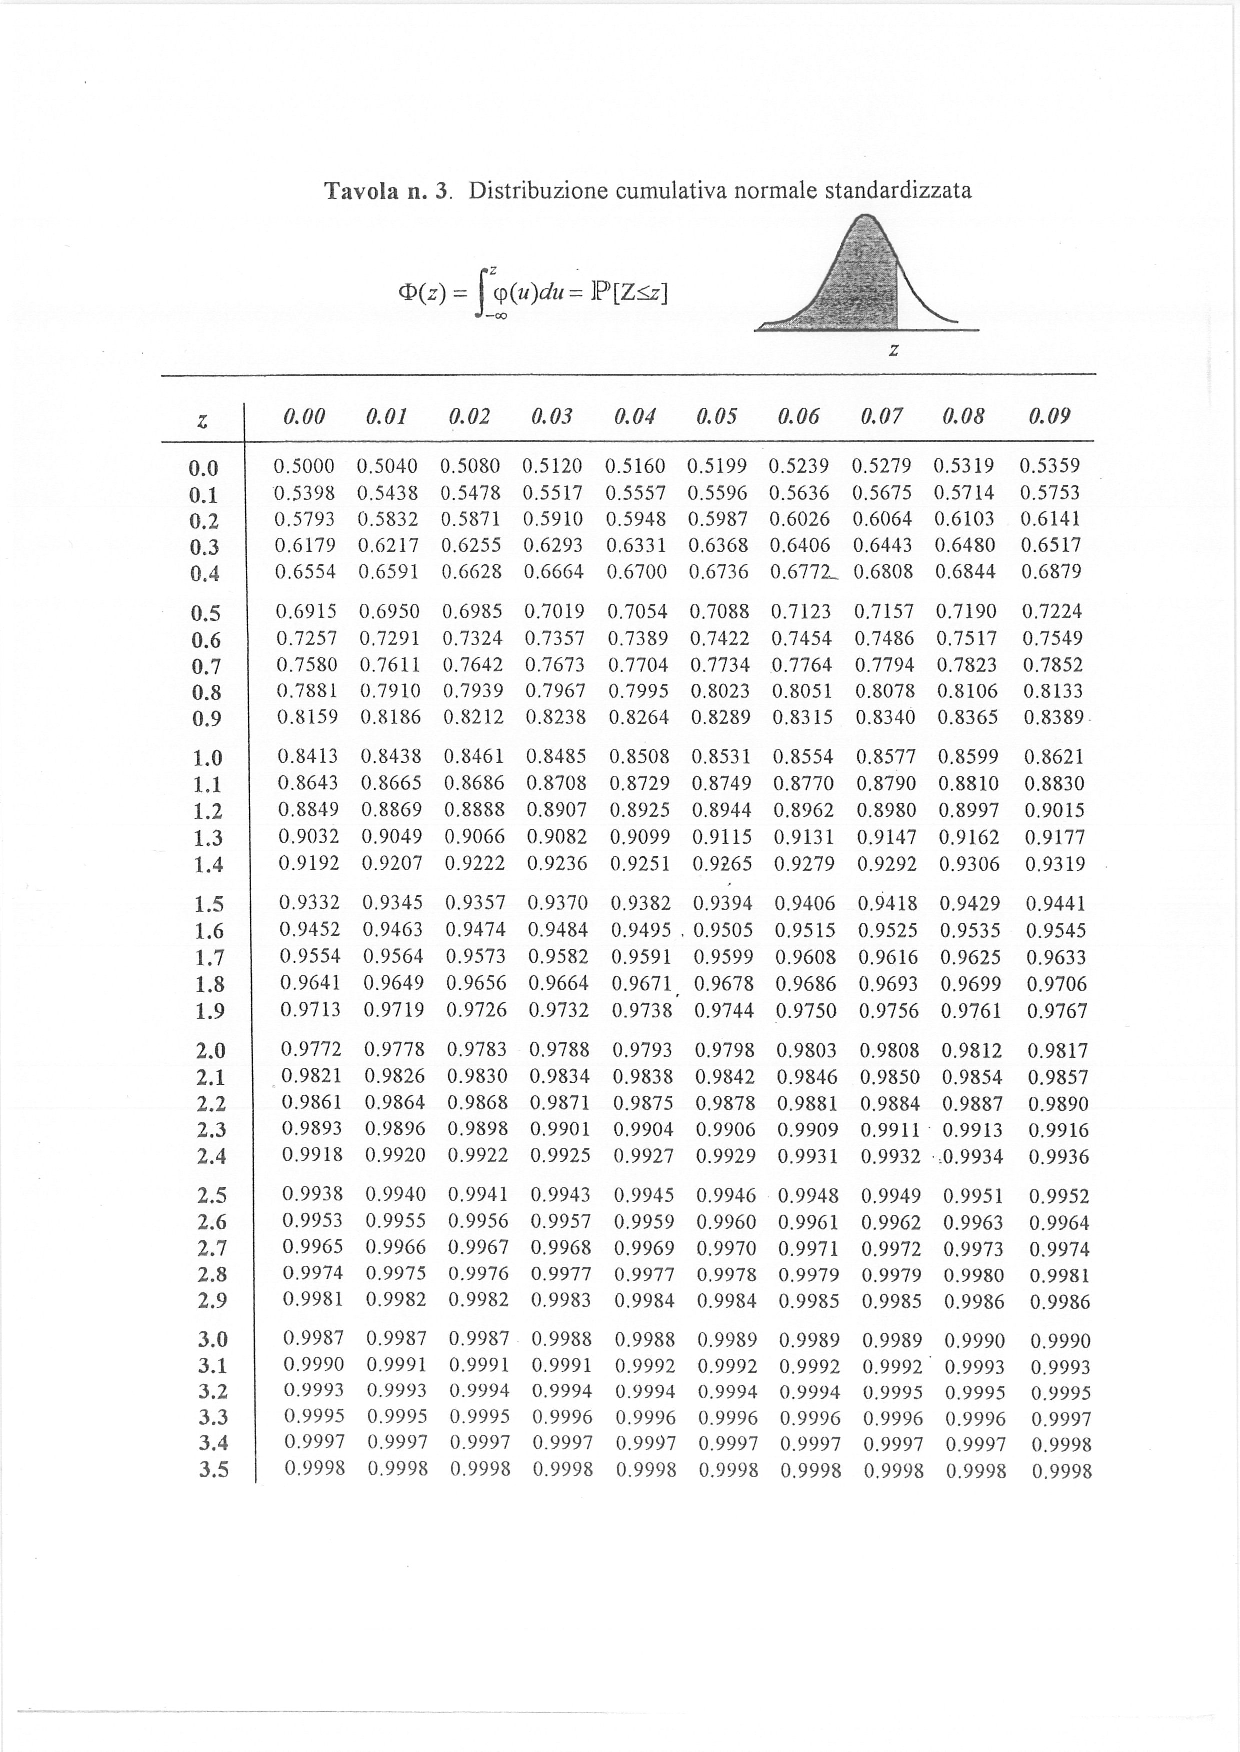
\includepdf[pages=-]{tavola normale.pdf}


\includepdf[pages=3-6]{Tavole statistiche.pdf}

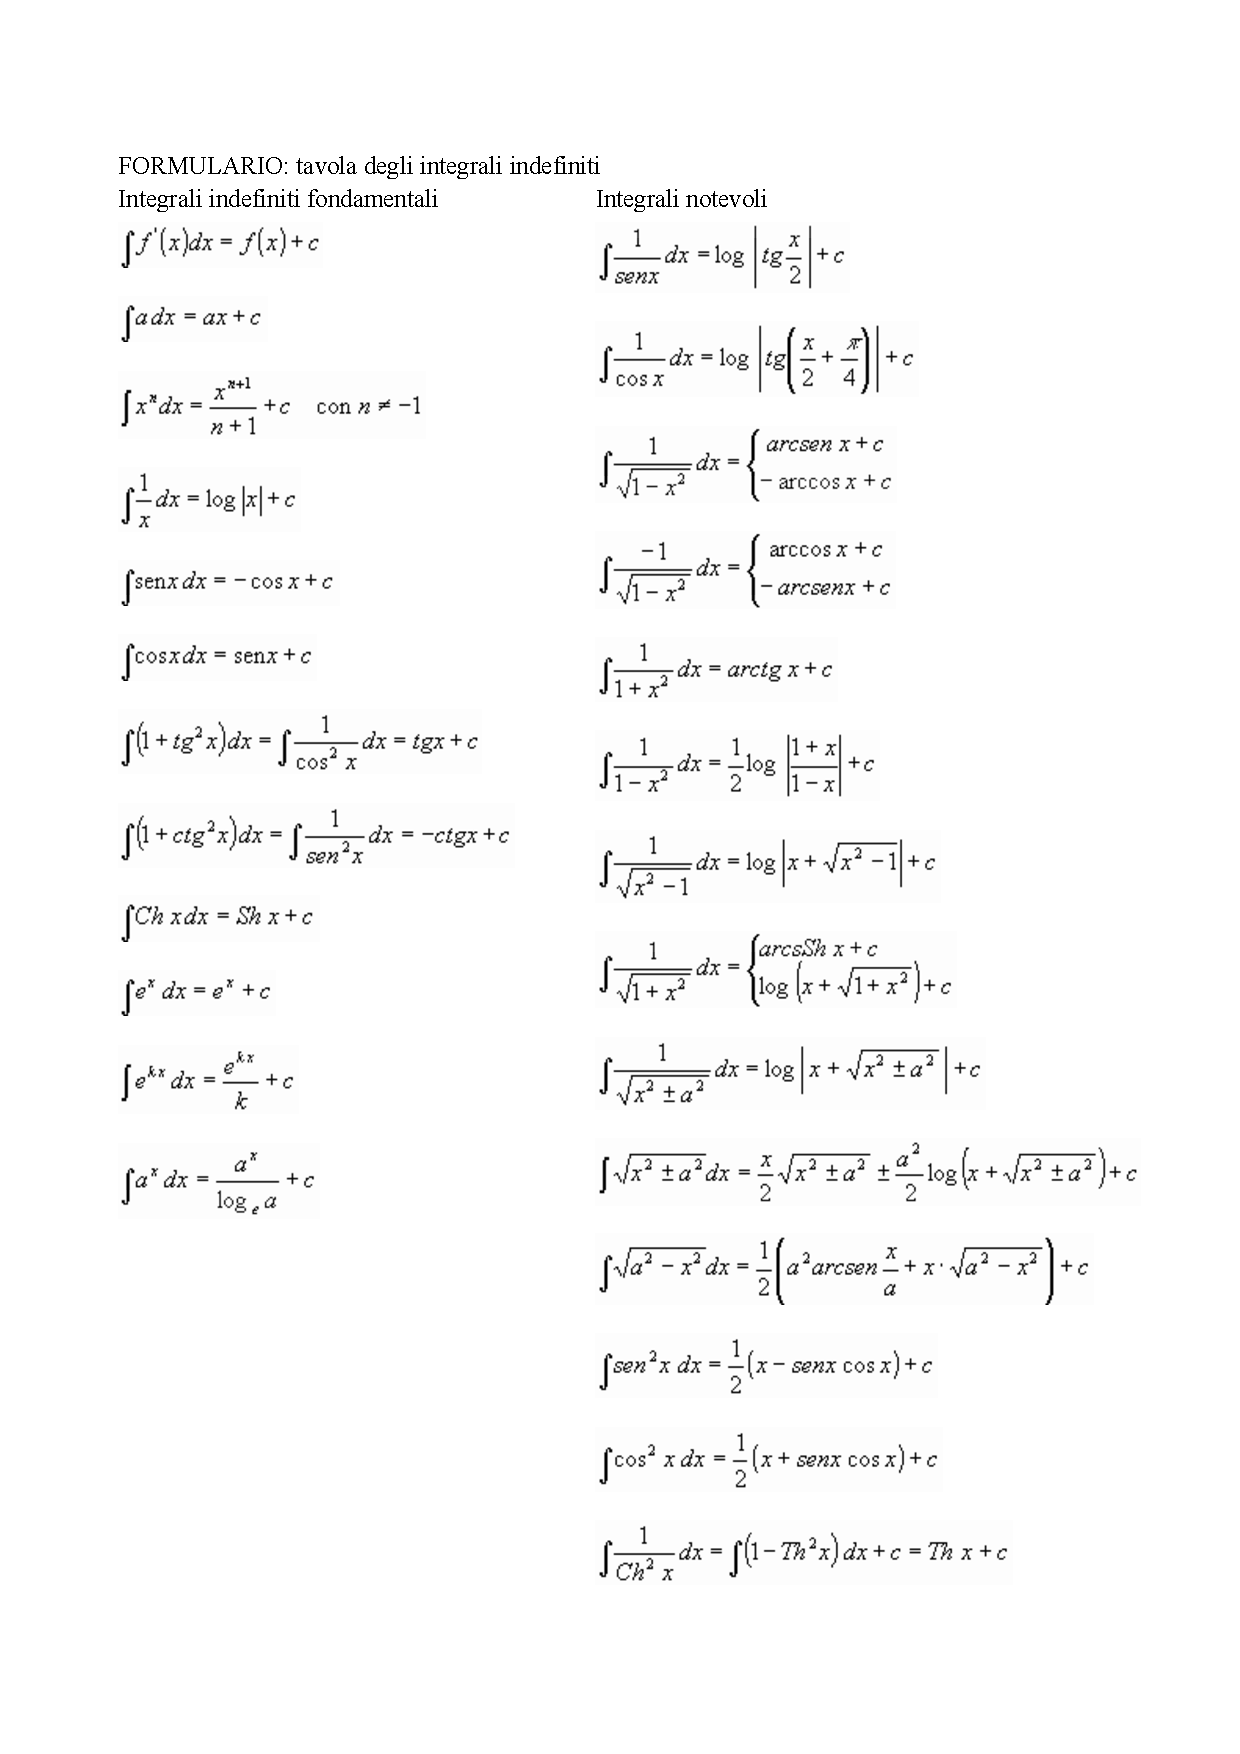
\includepdf[pages=1]{FORMULARIO INTEGRALI.pdf}

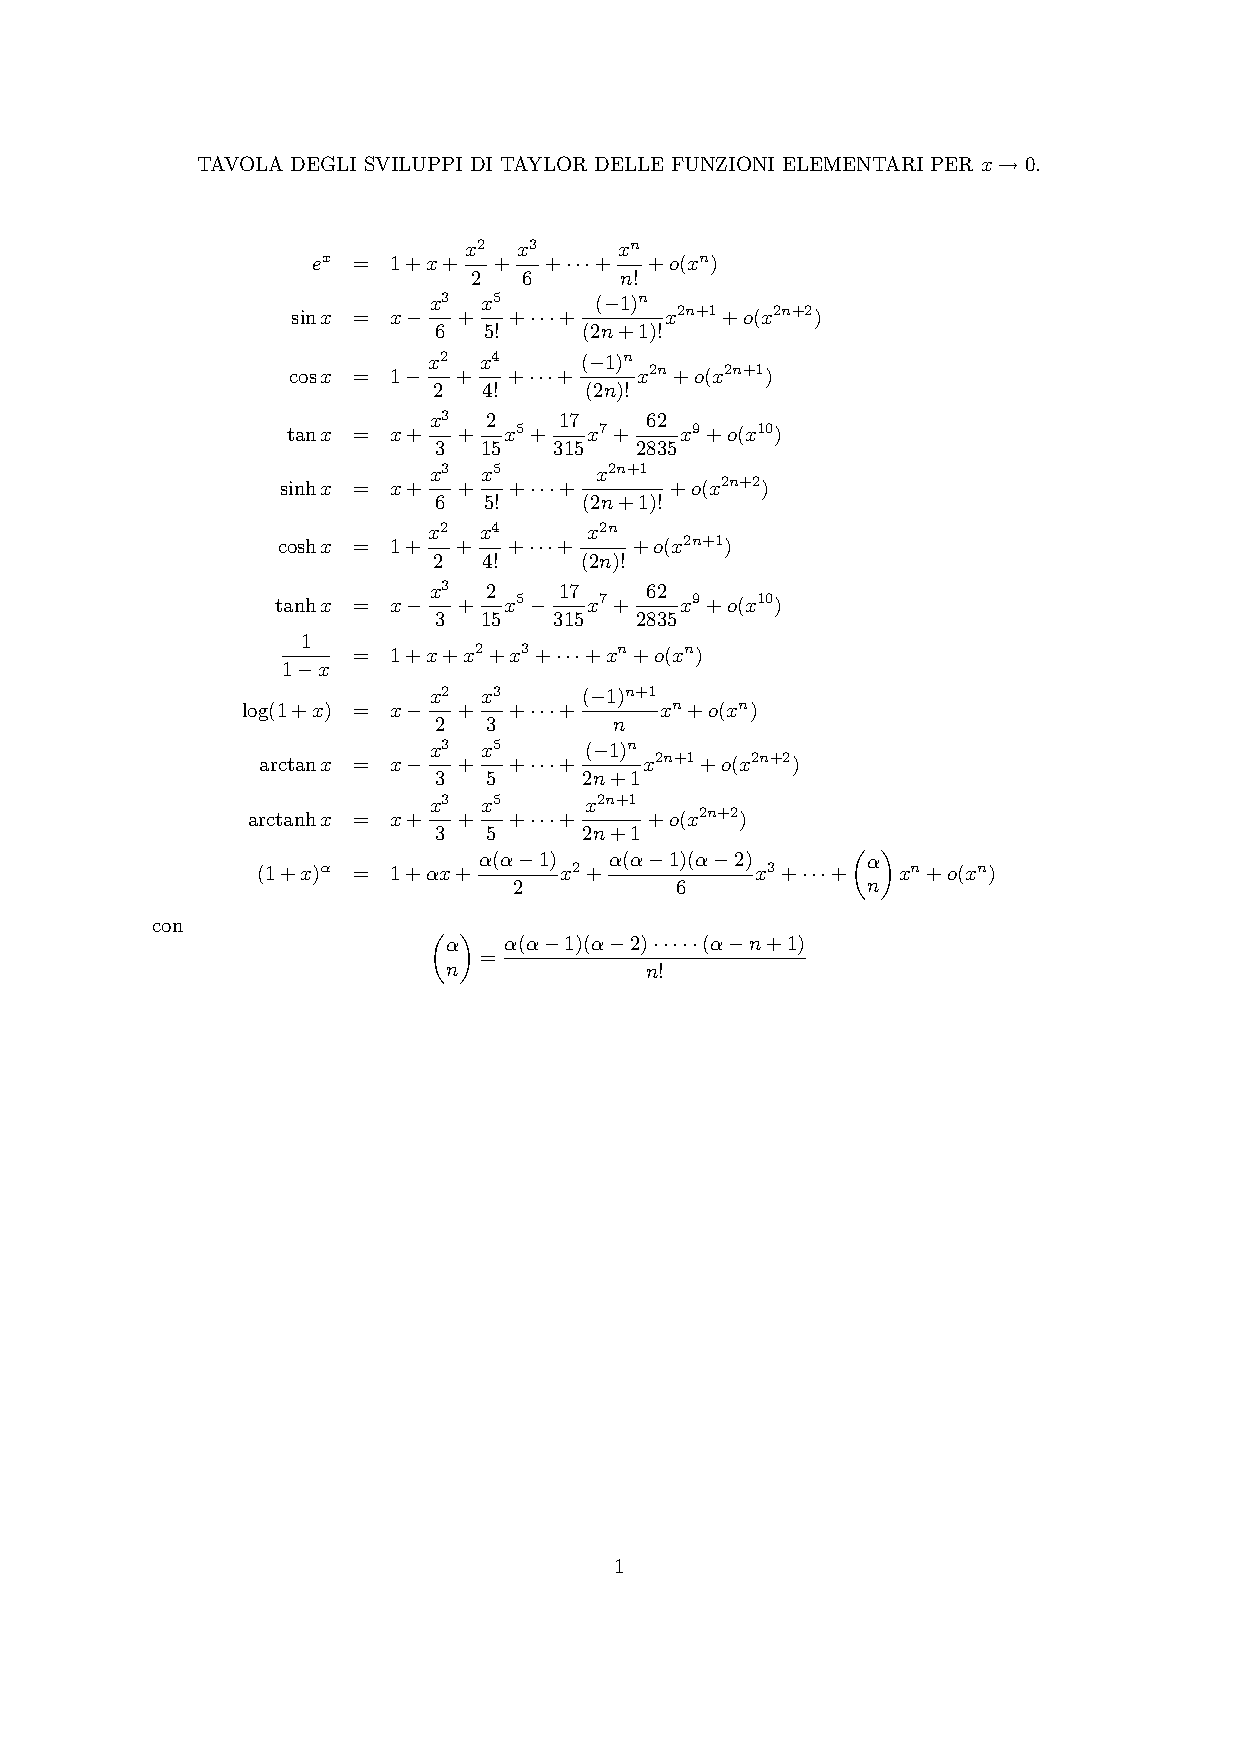
\includepdf[pages=1]{Sviluppi Taylor.pdf}

\end{document}
